\textbf{4.} \textbf{(2pts.)} Considera el siguiente fragmento de c\'odigo:
\begin{lstlisting}
if ( c[i] != 0 )
then 
   a[i] := b[i] / c[i];
else 
   a[i] := b[i];
\end{lstlisting}
Obtener las representaciones intermedias correspondientes a 1) \'arbol de 
sintaxis abstracta; 2) gr\'afica de control de flujo y 3) c\'odigo de tres 
direcciones. Explica tus respuestas. \\
Discutir (ampliamente) las ventajas que consideras para cada representaci\'on.

\begin{center}

    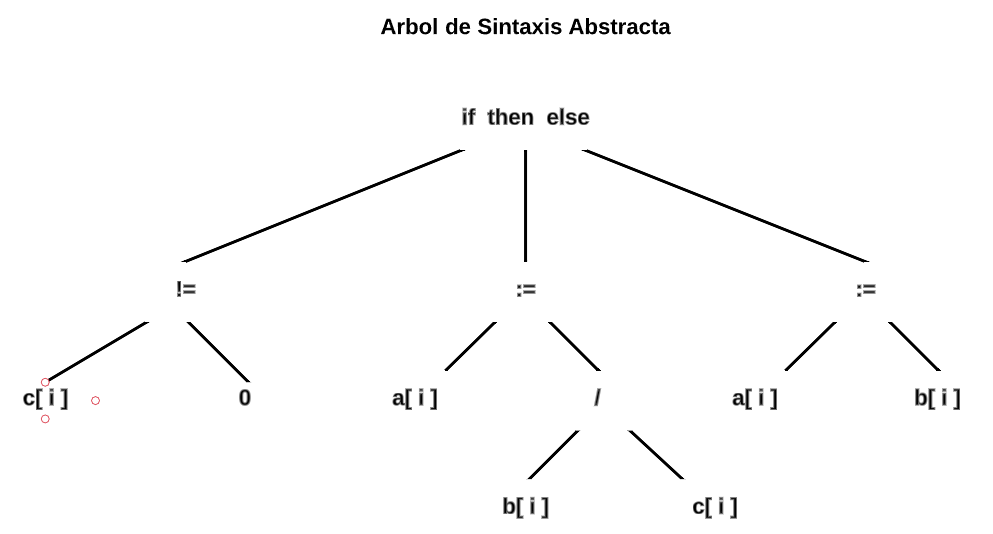
\includegraphics[scale = 0.5]{4_1}
    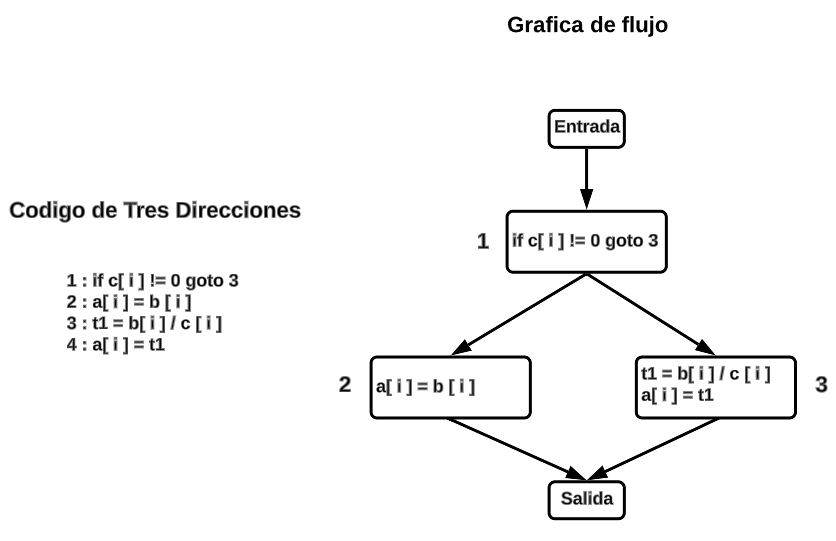
\includegraphics[scale = 0.5]{4_2}

 \end{center}

\textbf{Árbol de sintaxis abstracta}
\begin{enumerate}
    \item Representación estructural: Genera una representación estructural del código, capturando la jerarquía y las relaciones entre diferentes construcciones del lenguaje.
    Preserva la estructura sintáctica y semántica del código.
    \item Independencia del lenguaje: Es independiente del lenguaje y se puede utilizar como una representación intermedia en compiladores para varios lenguajes de programación.
    \item Facilidad de manipulación: Permite recorrer y manipular fácilmente mediante algoritmos y transformaciones.
    Facilita el análisis, optimización y transformación del código fuente.
    \item Detección de errores: Ayuda a detectar y reportar errores de sintaxis, errores de tipo y otros problemas semánticos durante el proceso de compilación.
\end{enumerate}

\textbf{Gráficos de flujo}
\begin{enumerate}
    \item Análisis de flujo de control: Proporciona una representación clara y visual del flujo de control dentro de un programa.
    Ayuda a analizar las rutas de ejecución del programa, detectar bucles, identificar código inaccesible y realizar transformaciones de programa relacionadas con el flujo de control.
    \item Optimización de rendimiento: Puede ser utilizado para optimizar el código, como identificar oportunidades para desenrollar bucles, fusionar bucles o mover código invariante al bucle.
    \item Depuración y perfilado: Ayuda en la depuración y el perfilado del programa al proporcionar información sobre el flujo de control, lo que permite comprender el comportamiento del programa e identificar cuellos de botella de rendimiento.
\end{enumerate}

\textbf{Código de tres direcciones}
\begin{enumerate}
    \item Representación de bajo nivel: Es una representación de bajo nivel que simplifica construcciones complejas de lenguajes de alto nivel en operaciones básicas con direcciones explícitas.
    Abstrae los detalles específicos del lenguaje y se centra en operaciones esenciales.
    \item Optimización de código: También sirve como una representación intermedia que permite diversas optimizaciones de código, como la reducción de constantes, la eliminación de subexpresiones comunes y la asignación de registros.
    \item Generación de código: Puede ser utilizada como entrada para generar código máquina, apuntando a arquitecturas específicas o máquinas virtuales.
    \item Modularidad: Facilita transformaciones y optimizaciones modulares en operaciones individuales o bloques de código sin afectar la estructura completa del programa.
\end{enumerate}